\documentclass{article}
\usepackage{graphicx} % Required for inserting images
\usepackage{listings} % Required for coding
\usepackage{xcolor}
\usepackage{amsmath}
\usepackage{amssymb}
\usepackage{placeins}
\usepackage{setspace}
\usepackage{tikz}
\usetikzlibrary{shapes.geometric, arrows}
\usepackage{cite}
\tikzstyle{startstop} = [rectangle, rounded corners, minimum width=3cm, minimum height=1cm,text centered, draw=black, fill=red!30]
\tikzstyle{process} = [rectangle, minimum width=3cm, minimum height=1cm, text centered, draw=black, fill=orange!30]
\tikzstyle{arrow} = [thick,->,>=stealth]

\usepackage{algorithm}
\usepackage{algorithmic}
\usepackage{subcaption}
\usepackage{tikz}
\usetikzlibrary{matrix, positioning}
\usetikzlibrary{matrix}
\title{m2r Group45}
\author{rongzhi zhu}
\date{June 2024}
\usepackage[a4paper,top=1in,bottom=1in,left=1in,right=1in,marginparwidth=1.75cm]{geometry}

\usepackage{setspace}
\usepackage{tikz}
\usetikzlibrary{shapes.geometric, arrows}

\tikzstyle{startstop} = [rectangle, rounded corners, minimum width=3cm, minimum height=1cm,text centered, draw=black, fill=red!30]
\tikzstyle{process} = [rectangle, minimum width=3cm, minimum height=1cm, text centered, draw=black, fill=orange!30]
\tikzstyle{arrow} = [thick,->,>=stealth]

\begin{document}
\doublespacing

\subsection{Traditional Compression Method}
This part is a brief explanation about how to build a contraction for an image in traditional way. The image could be not self-similar.
\subsubsection{Introduction of Theory}

Firstly, for compressing a image, we need to define the metric first. The metric including the image set E and distance d. We define the image set as \( E = [0,1]^{h \times w} \), which is a matrix with \( h \) rows and \( w \) columns, and each entry is a number in the range \([0,1]\). Also, the distance \( d \) is defined as the Frobenius norm:
\[
d(x, y) = \sqrt{\sum_{i=1}^{h} \sum_{j=1}^{w} (x_{ij} - y_{ij})^2}
\]

Secondly, we segment the image into two different ways: Domain blocks and Range blocks. We divide the image into Domain blocks (D) and Range blocks (R) to more effectively find the best matches and achieve image compression. The role of D blocks is to provide potential matching sources. Each domain block can generate multiple candidate blocks through a series of transformations (such as scaling, rotating, flipping, adjusting contrast, and brightness), which are then compared with R blocks. Since D blocks serve as sources for matching, they do not need to be disjoint, nor do they need to cover the entire image.
R blocks are the target blocks that need to be compressed. Each R block will search for the best matching D block and the corresponding transformation to accurately represent the content of the original image. Because we need to ensure that all image information is considered and compressed, range blocks must be disjoint and cover the entire image. Using transformed D blocks to represent range blocks achieves image compression.

In conclusion, domain blocks are divided into \( D_1, D_2, \ldots, D_k \). These sub-blocks are not necessarily disjoint and they do not need to cover the image. Range blocks are divided into \( R_1, R_2, \ldots, R_L \). These sub-blocks need to be disjoint and cover the whole image.

Finally, for each range block \( R_l \), we will choose a domain block \( D_{k_l} \) and a mapping \( f_l : [0, 1]^{D_{k_l}} \rightarrow [0, 1]^{R_l} \). Then, we can define our function \( f \) as:
\[
f(x)_{ij} = f_l(x_{D_{k_l}})_{ij} \quad \text{if } (i,j) \in R_l
\]
( If all \( f_l \) are contractions then \( f \) is a contraction.)




\subsubsection{Implementation}
In this section, we will explain the entire algorithm used to compress images.

\paragraph{Segmentation}

The domain block is divided into 8 by 8, and the range blocks are 4 by 4.
This is just one way for segmentation. There is other ways to segment, such as guadtree-based fractal encoding scheme.
% Figure 1: Domain and Range blocks
\begin{figure}[ht]
    \centering
    \begin{subfigure}[b]{0.45\textwidth}
        \centering
        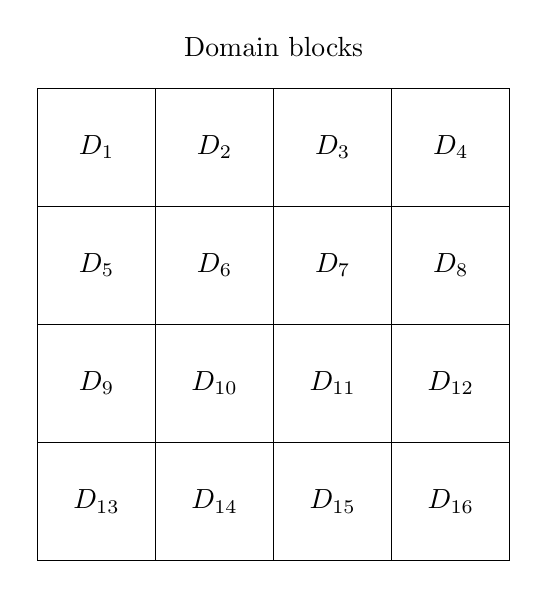
\begin{tikzpicture}
        % Domain blocks
        \matrix (m1) [matrix of nodes, nodes={draw, minimum size=1.5cm, anchor=center}, column sep=-\pgflinewidth, row sep=-\pgflinewidth] {
            $D_1$ & $D_2$ & $D_3$ & $D_4$ \\
            $D_5$ & $D_6$ & $D_7$ & $D_8$ \\
            $D_9$ & $D_{10}$ & $D_{11}$ & $D_{12}$ \\
            $D_{13}$ & $D_{14}$ & $D_{15}$ & $D_{16}$ \\
        };
        \node at (m1.north) [above=1ex] {Domain blocks};
        \end{tikzpicture}
        \caption{Domain blocks}
    \end{subfigure}
    \hfill
    \begin{subfigure}[b]{0.45\textwidth}
        \centering
        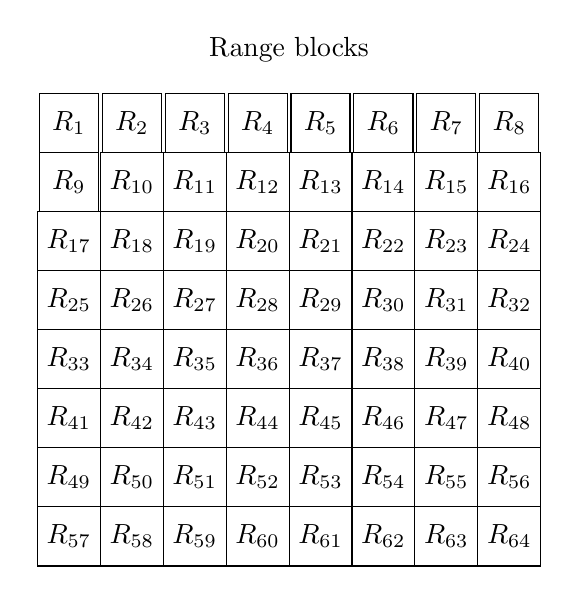
\begin{tikzpicture}
        % Range blocks
        \matrix (m2) [matrix of nodes, nodes={draw, minimum size=0.75cm, anchor=center}, column sep=-\pgflinewidth, row sep=-\pgflinewidth] {
            $R_1$ & $R_2$ & $R_3$ & $R_4$ & $R_5$ & $R_6$ & $R_7$ & $R_8$ \\
            $R_9$ & $R_{10}$ & $R_{11}$ & $R_{12}$ & $R_{13}$ & $R_{14}$ & $R_{15}$ & $R_{16}$ \\
            $R_{17}$ & $R_{18}$ & $R_{19}$ & $R_{20}$ & $R_{21}$ & $R_{22}$ & $R_{23}$ & $R_{24}$ \\
            $R_{25}$ & $R_{26}$ & $R_{27}$ & $R_{28}$ & $R_{29}$ & $R_{30}$ & $R_{31}$ & $R_{32}$ \\
            $R_{33}$ & $R_{34}$ & $R_{35}$ & $R_{36}$ & $R_{37}$ & $R_{38}$ & $R_{39}$ & $R_{40}$ \\
            $R_{41}$ & $R_{42}$ & $R_{43}$ & $R_{44}$ & $R_{45}$ & $R_{46}$ & $R_{47}$ & $R_{48}$ \\
            $R_{49}$ & $R_{50}$ & $R_{51}$ & $R_{52}$ & $R_{53}$ & $R_{54}$ & $R_{55}$ & $R_{56}$ \\
            $R_{57}$ & $R_{58}$ & $R_{59}$ & $R_{60}$ & $R_{61}$ & $R_{62}$ & $R_{63}$ & $R_{64}$ \\
        };
        \node at (m2.north) [above=1ex] {Range blocks};
        \end{tikzpicture}
        \caption{Range blocks}
    \end{subfigure}
    \caption{Domain and Range blocks}
    \label{fig:blocks}
\end{figure}

% Figure 2: Quadtree-based fractal encoding scheme
\begin{figure}[ht]
    \centering
    \includegraphics[width=0.3\textwidth]{pic3}
    \caption{Quadtree-based fractal encoding scheme}
    \label{fig:quadtree}
\end{figure}

\paragraph{Transformation}
In this section, we attempt to construct the contraction mappings from \( D_k \) to \( R_l \). Our goal is to generate a mapping \( f_l \) such that \( f(x_{D_k}) \) is close to \( x_{R_l} \). In other words, we hope to find a mapping that makes \( D_k \) and \( R_l \) very similar after the transformation. Clearly, the more mappings we generate, the more likely we are to find a good one. However, if we have a set of functions \( f_l \) that is too large, the compression efficiency will deteriorate. Thus, there is a tradeoff: the more mappings we have, the better the potential matches, but at the cost of more storage space required for the mappings.

The mapping we choose here has the following form:
\[
f_l (x_{D_k}) = s \times \text{rotate}_\theta (\text{flip}_d (\text{reduce}(x_{D_k}))) + b
\]

And here is the pseudo code of how to apply transformation.
\begin{algorithm}
\caption{Apply Transformation}
\begin{algorithmic}[1]
\REQUIRE img, direction, angle, contrast = 1.0, brightness = 0.0
\STATE // Apply flipping, rotating, contrast adjustment, and brightness adjustment
\STATE transformed\_img = flip(img, direction)
\STATE // Flip the image horizontally or vertically based on direction
\STATE transformed\_img = rotate(transformed\_img, angle)
\STATE // Rotate the image by a given angle (90, 180, 270 degrees)
\STATE transformed\_img = contrast * transformed\_img + brightness
\RETURN transformed\_img
\end{algorithmic}
\end{algorithm}


\subsubsection{Compression}
After determining the method of transformation, we need to start compressing the image. According to the previous approach, we first generate all affine transformations of the domain blocks. Then, for each range block, we find the best corresponding domain block and optimize its contrast and brightness. Finally, we return the best transformation parameters for all range blocks to achieve image compression.

% Generate transformed blocks
\begin{algorithm}
\caption{Generate All Transformed Blocks}
\begin{algorithmic}[1]
\REQUIRE img, source\_size, destination\_size, step
\STATE factor $\gets$ source\_size // destination\_size \textcolor{gray}{// Calculate scaling factor}
\STATE transformed\_blocks $\gets$ empty list \textcolor{gray}{// Initializes an empty list to store all the transformed blocks}
\FOR{each source block in img}
    \STATE S $\gets$ reduce(source block, factor) \textcolor{gray}{// Reduce source block}
    \FOR{each transformation in candidates}
        \STATE transformed $\gets$ apply\_transform(S, transformation) % Apply transformation
        \STATE add (position, transformation, transformed) to transformed\_blocks \textcolor{gray}{//Add transformation info into transformed blocks}
    \ENDFOR
\ENDFOR
\RETURN transformed\_blocks
\end{algorithmic}
\end{algorithm}

% Explanation of the compression process
Following is the \texttt{compress} function. It iterates over each destination block in the image, extracts it, and tests all the previously generated transformed source blocks to find the best match. The best match is determined by optimizing the contrast and brightness using the \texttt{find\_contrast\_and\_brightness2} function, which solves a least squares problem to fit the contrast and brightness. The function returns the best transformation parameters for all destination blocks, achieving image compression.

\begin{algorithm}
\caption{Compress Image}
\begin{algorithmic}[1]
\REQUIRE img, source\_size, destination\_size, step
\STATE transformations $\gets$ empty list
\STATE transformed\_blocks $\gets$ generate\_all\_transformed\_blocks(img, source\_size, destination\_size, step)
\FOR{each destination block position (i, j) in img}
    \STATE add empty list to transformations[i]
    \STATE min\_d $\gets$ infinity
    \STATE D $\gets$ extract\_destination\_block(img, i, j, destination\_size) \textcolor{gray}{//D is the destination block}
    \FOR{each transformed block in transformed\_blocks}
        \STATE S $\gets$ transformed block \textcolor{gray}{//Now S is the new transformed block}
        \STATE (contrast, brightness) $\gets$ find\_contrast\_and\_brightness2(D, S) \textcolor{gray}{//Find the best contrast and brightness for S and D}
        \STATE S $\gets$ contrast $\times$ S + brightness \textcolor{gray}{//Adjust S}
        \STATE d $\gets$ compute\_difference(D, S) \textcolor{gray}{//Compute difference}
        \IF{d \textless  min\_d}
            \STATE min\_d $\gets$ d
            \STATE transformations[i][j] $\gets$ (k, l, direction, angle, contrast, brightness) \textcolor{gray}{//Save the best transformation parameters for current D}
        \ENDIF
    \ENDFOR
\ENDFOR
\RETURN transformations
\end{algorithmic}
\end{algorithm}

\FloatBarrier
\subsubsection{Decompression}


\begin{algorithm}
\caption{Decompress Image}
\begin{algorithmic}[1]
\REQUIRE transformations, source\_size, destination\_size, step, nb\_iter=8
\STATE factor $\gets$ \texttt{source\_size // destination\_size} \textcolor{gray}{// Calculate scaling factor}
\STATE height $\gets$ \texttt{len(transformations) $\times$ destination\_size} \textcolor{gray}{// Image height}
\STATE width $\gets$ \texttt{len(transformations[0]) $\times$ destination\_size} \textcolor{gray}{// Image width}
\STATE iterations $\gets$ [\texttt{np.random.randint(0, 256, (height, width))}] \textcolor{gray}{// Initial random image}
\STATE cur\_img $\gets$ \texttt{np.zeros((height, width))} \textcolor{gray}{// Initialize current image}
\FOR{i\_iter $\gets$ 0 \textbf{to} nb\_iter}
    \FOR{i $\gets$ 0 \textbf{to} \texttt{len(transformations)}}
        \FOR{j $\gets$ 0 \textbf{to} \texttt{len(transformations[i])}}
            \STATE (k, l, flip, angle, contrast, brightness) $\gets$ transformations[i][j] \textcolor{gray}{// Get transformation}
            \STATE Reduce the source block \textcolor{gray}{// Reduce block}
            \STATE Apply the transformation \textcolor{gray}{// Apply transform}
            \STATE Update the current image \textcolor{gray}{// Update image}
        \ENDFOR
    \ENDFOR
    \STATE Save the current image \textcolor{gray}{// Save iteration}
    \STATE Reset the current image \textcolor{gray}{// Reset image}
\ENDFOR
\RETURN iterations \textcolor{gray}{// Return iterations}
\end{algorithmic}
\end{algorithm}


\subsection{issue and idea of improvement}

The theoretical basis of fractal compression methods is Iterated Function Systems (IFS) theory. However, this methods also has several disadvantages:

1. \textbf{Long Encoding Time}: The extensive search and matching required for encoding lead to long processing times.

2. \textbf{Lower Compression Ratio}: The compression ratio is not as high because the method does not comprehensively consider global and local similarities. This limitation results in significant constraints in simple block-to-block transformations.

To address these disadvantages, improvements can be focused on the following areas:

1. \textbf{Enhancing Compression Ratio and Compression Effect}: By developing more sophisticated algorithms that better capture the similarities within and across frames, the compression ratio and overall effect can be improved.

2. \textbf{Increasing Encoding Speed}: Optimization techniques such as parallel processing, more efficient search algorithms, and hardware acceleration can significantly reduce encoding times.

3. \textbf{Increasing Decoding Speed}: Similar optimization techniques can also be applied to the decoding process to enhance its speed.

4. \textbf{Combining with Other Methods}: Integrating fractal coding with other compression methods can leverage the strengths of both approaches, potentially overcoming the limitations of each.

\subsubsection{Enhancing Compression Ratio and Compression Effect}

According to theoretical analysis, the size of the domain blocks and range blocks has a significant impact on the quality and compression ratio of fractal image coding. Considering two extreme cases: if the domain block is \(2^D \times 2^D\) pixels and the range block is \(2^R \times 2^R\) pixels, when \(D\) and \(R\) are very large, although the number of domain blocks in the domain block library is relatively large, it is difficult to find a high similarity between the range block and the domain block, resulting in poor image quality after decoding. Conversely, if \(D\) and \(R\) are very small, the smallest case being a range block of one pixel and a domain block of four pixels, it is always possible to find a very good similarity match coefficient, but the number of affine transformations required for image coding increases sharply, failing to achieve the purpose of compression.\\
Therefore, Fisher and Jacquin proposed an adaptive adjustment method, which improves the coding effect and compression ratio by changing the size of the range blocks and domain blocks. The key to this method is to use a tolerable error (\( \varepsilon \)) to decide the size adjustment of the blocks.


\textbf{Adaptive Quadtree Coding Method}

1. \textbf{Adjusting Block Size}
   \begin{itemize}
       \item For large domain blocks and range blocks, choose appropriate affine transformation coefficients.
       \item For large blocks where a good match cannot be found, progressively reduce the block size from \( 2^R \) to \( 2^{R-1} \), \( 2^{R-2} \), and so on.
   \end{itemize}

2. \textbf{Error and Compression Ratio}
   \begin{itemize}
       \item Match blocks by allowing a certain error \( \varepsilon \).
       \item If the tolerable error is large, the compression ratio is high but the image quality may be poor; if the tolerable error is small, the compression ratio is low but the image quality is good.
   \end{itemize}

\begin{enumerate}
    \item \textbf{Initial Block Division}: Divide the image into initial large blocks.
    \item \textbf{Matching and Adjustment}: For each large block, search for the best matching domain block. If no suitable match is found, subdivide the block into smaller blocks and repeat the process.
    \item \textbf{Affine Transformation}: Calculate the corresponding affine transformation parameters for each matched block and use these parameters for coding.
    \item \textbf{Error Calculation}: Calculate the matching error for each iteration to ensure it is within the allowable range.
\end{enumerate}

Here is a citation to the article: \cite{may1996fractal}.
%%%%%%%%%%%%%%%%%%%%%%%%%%%%%%%%%%%%%
\nocite{*}
\bibliographystyle{plain}
\bibliography{ref}
\end{document}